%#!platex Naruse_Esurf_2020.tex

\section{Results}

\subsection{Properties of artificial data sets of turbidites}
Here, we describe the properties of turbidite artificial data generated for training and testing the inverse model. Several artificial datasets of turbidites are produced using a 1-D shallow water equation model. Figure \ref{fig:training_examples_artificial_turbidites} exhibits examples of the calculated spatial distribution in bed thickness and grain size of turbidites deposited in the region of the basin plain. Most beds exhibit the typical ``top-hat'' or ``core and drape'' shape of turbidites \cite{Hirayama1977,Talling2012,Pantopoulos2013}, where turbidite beds become thicker in the upstream part of the basin and then thin rapidly from their peak of thickness. Thereafter, beds continue over a long distance, gradually decreasing in thickness (Fig. \ref{fig:training_examples_artificial_turbidites}). At the same time, the grain size gradually becomes finer downstream. The maximum thickness of beds is 1.27 m on average (standard deviation $\sigma = 1.65$ m), and the mean value of the area where sediments with a thickness greater than 1 cm are distributed is 42.0 km ($\sigma=15.7$ km). 

The vertically averaged grain size at the upstream end of the sedimentary basin in each bed was 1.9 phi on average, and the mean grain size in the entire basin plain was 2.5 phi. 

\begin{figure}[t]
  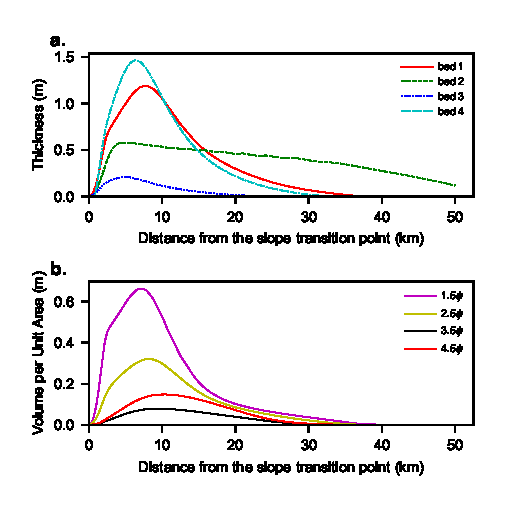
\includegraphics[width=8cm]{fig04.eps}
  \caption{Examples of turbidites calculated by the forward model. \textsf{a}. Spatial distributions of bed thickness. Four beds (Bed 1--4) were plotted as examples. \textsf{b}. Spatial distribution of the volume-per-unit-area for each grain size class in Bed 1 (Fig. 4a).}
  \label{fig:training_examples_artificial_turbidites}
\end{figure}

\subsection{Results of training}
We trained the NN inverse model with various numbers of artificial data and lengths of the sampling window, and the best result in terms of the value of the loss function for the validation sets and the practical usage of the model can be obtained with 3500 training data sets and 10 km-long sampling window  (Fig. \ref{fig:training_different_number_length}). Results with less than 2000 training data sets produce a discrepancy in the loss function between the training and the validation sets, indicating overlearning of the NN. Conversely, when the number of data sets exceeds 2000, the loss function of the validation set is slightly less than the value of the training set. As the number of training data increases, the resultant values of the loss function improve. However, when the number of data exceeds 2500, the improvement of values of the loss function became not so rapid. Regarding the distance of the sampling window, the training results are not stable when the sampling window is shorter than 5 km (Fig. \ref{fig:training_different_number_length}). On the other hand, the training results are stable when the window length is longer than 10 km, and the results gradually improve as the window length increases. However, extending the window length from 10 km to 30 km results in little improvement of the loss function. 

\begin{figure}[t]
  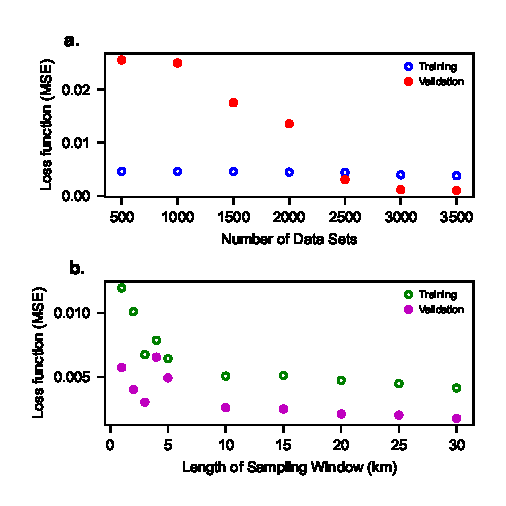
\includegraphics[width=8cm]{fig05.eps}
  \caption{Results of training of the NN with different numbers of training data sets and lengths of the sampling window.}
  \label{fig:training_different_number_length}
\end{figure}

Hereafter, we further investigate the performance of the inverse model trained on a 3500 dataset with a 10 km-long sampling window. The history of training indicates that the values of the loss function improved significantly in the first 1000 epochs, and the results are improved up to 15,000 epochs (Fig. \ref{fig:training_history}). Eventually, saturation is reached at approximately 20,000 epochs. The resultant loss function (i.e., the MSE of prediction) is $3.78 \times 10^{-3}$ for training sets and is $1.03 \times 10^{-3}$ for validation sets.

\begin{figure}[t]
  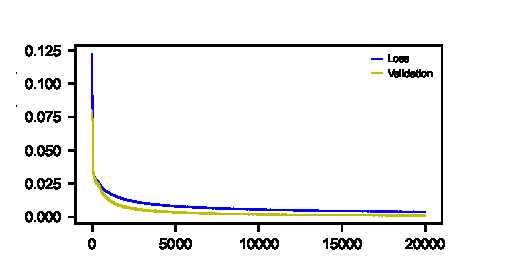
\includegraphics[width=8cm]{fig06.eps}
  \caption{Training History of the NN. 3500 datasets and 10 km-long sampling window were used for this training.}
  \label{fig:training_history}
\end{figure}


\subsection{Precision and accuracy of inverse analysis}
Using 300 test data sets, the performance of the inverse model trained with 3500 data sets and 10 km-long sampling window is evaluated. The estimated parameters are matched well with slight deviations (Figs. \ref{fig:test_scatter_plot}, \ref{fig:test_histogram_deviation}; Table \ref{table:bias_errors}). $R^2$ values are beyond 0.98 for all parameters. Particularly good agreement is obtained for the estimates of the initial height and the length of the suspended sediment cloud. Values of the normalized RMSE and MAE for these parameters are less than 9 \% and 6 \%, respectively. The sediment concentration is also precisely estimated. the normalized RMSE for the sediment concentration ranges from 12 to 16 \%, which corresponds to only 0.02--0.03 volumetric \%. The prediction for the basin slope shows relatively large errors (RMSE is close to 20 \% and MAE is 11.7 \%), but these errors correspond to only 0.03 \% of slope. Focusing on the bias of the estimates, all estimated values except for the basin slope tend to be slightly smaller, whereas the predicted values of the basin slope tend to be  larger (Fig. \ref{fig:test_histogram_deviation}). The values of the bias, however, range only from 2 to 12\% of the original value. 

\begin{figure*}[t]
  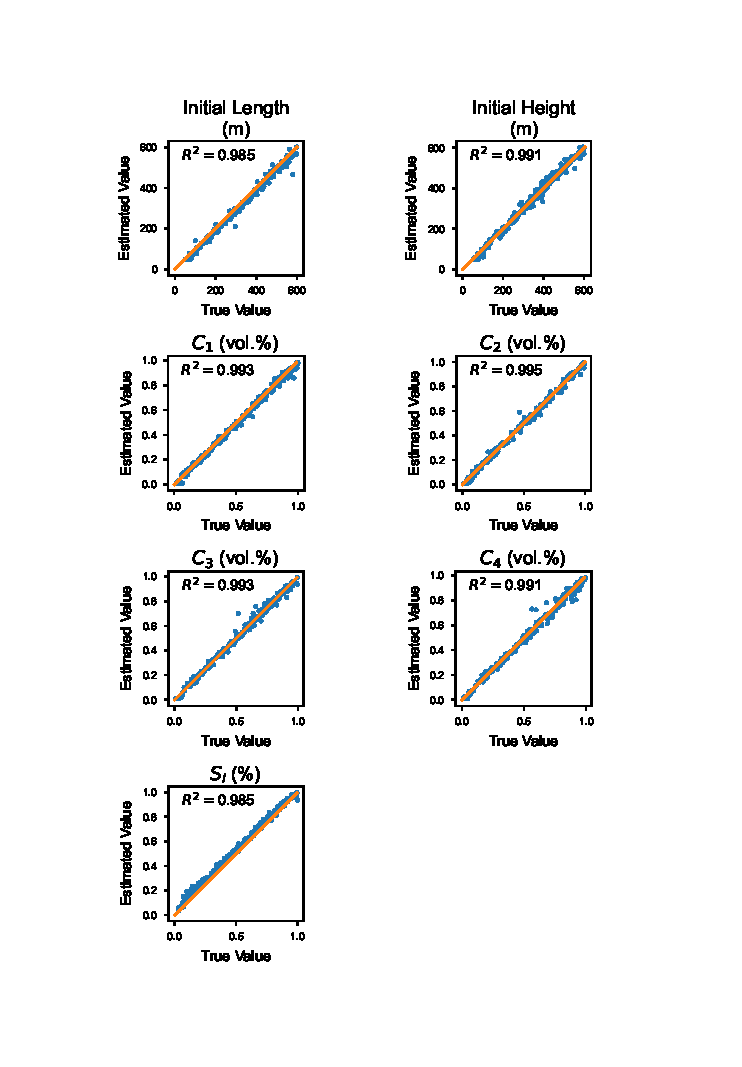
\includegraphics[width=12cm]{fig07.eps}
  \caption{Result of the inverse analysis compared with the true parameters. The x-axis represents the value of the true parameter and the y-axis represents the value of the estimated parameter. The orange lines show that the two values are in a 1:1 relationship, and thus the plots on this line indicate that the prediction is perfectly consistent with the true value.}
  \label{fig:test_scatter_plot}
\end{figure*}

\begin{figure*}[t]
  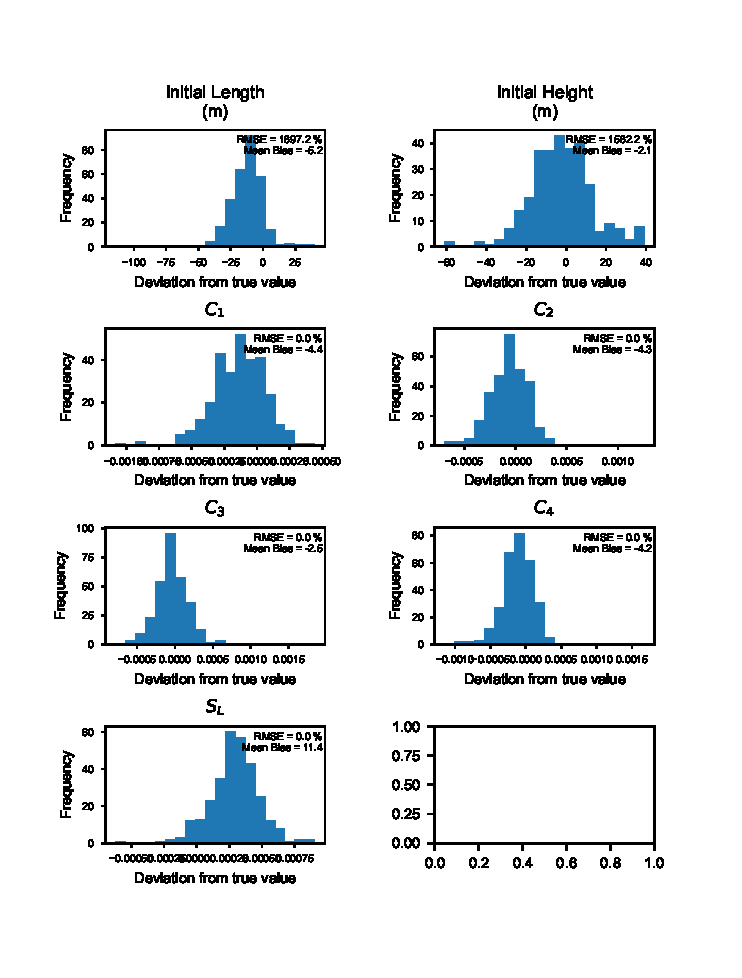
\includegraphics[width=12cm]{fig08.eps}
  \caption{Histograms indicating the deviation of the predicted values from the true values.}
  \label{fig:test_histogram_deviation}
\end{figure*}

\begin{table*}[t]
  \caption{Errors and bias of the predicted parameters. Prediction errors are exhibited by the root mean squared error (RMSE) and the mean absolute error (MAE), and the mean bias is also described. Normalized values of RMSE, MAE and mean bias by true values are also shown.}
  \begin{tabular}{lrrrrrrr}
    \hline
    {} &  $R^2$ &  RMSE &  \begin{tabular}{c} RMSE \\ (normalized) \end{tabular} &   MAE &  \begin{tabular}{c} MAE \\ (normalized) \end{tabular} &  Mean bias & \begin{tabular}{c} Mean bias \\(normalized) \end{tabular} \\
    \hline
    Initial height & 0.99 & 18.97 m &               8.55 \% & 14.81 m &              5.96 \%&     -12.93 m&                   -5.18 \%\\
Initial length & 0.99 & 15.82 m&               7.53 \%& 12.09 m&              4.92 \%&      -2.33 m&                   -2.06 \%\\
$C_1$            & 0.99 &  0.02 \%&              12.91 \%&  0.02 \%&              6.00 \%&      -0.01 \%&                   -4.44 \%\\
$C_2$            & 0.99 &  0.02 \%&              15.57 \%&  0.02 \%&              7.67 \%&      -0.01 \%&                   -4.29 \%\\
$C_3$            & 0.99 &  0.02 \%&              13.03 \%&  0.02 \%&              6.39 \%&      -0.00 \%&                   -2.49 \%\\
$C_4$            & 0.99 &  0.03 \%&              13.71 \%&  0.02 \%&              6.67 \%&      -0.01 \%&                   -4.21 \%\\
$S_l$            & 0.98 &  0.03 \%&              19.56 \%&  0.03 \%&             11.67 \%&       0.03 \%&                   11.45 \%\\
  \hline
    \end{tabular}
  \label{table:bias_errors}
\end{table*}


The forward model is calculated again using the reconstructed values to examine the influence of the estimation error of the model input parameters on the predicted flow behavior (Fig. \ref{fig:test_example_time_evolution}). The chosen test values deviate from the true conditions as indicated by the RMSE value 0.27 (Table \ref{table:example_time_evolution}), but the time evolution of the flow characteristics agree very well with those calculated from the true values (Fig. \ref{fig:test_example_time_evolution}). When comparing the velocity and concentration of the flow at 10 km from the upstream end, the discrepancy between calculation results using reconstructed and original parameters is less than 5\% for both parameters.

\begin{table*}[t]
  \caption{The predicted and the true parameters used for an example of calculation for time evolution of the flow characteristics.}
  \begin{tabular}{lrrrrrrr} \hline 
        {} &  Initial height (m) &  Initial length (m) &      $C_1$ &      $C_2$ &      $C_3$ &      $C_4$ &      $S_l$ \\
        \hline
        True input parameters &              484.41 &              318.18 &     0.17 &     0.05 &     0.95 &     0.74 &     0.23 \\
Estimated parameters  &              454.67 &              301.73 &     0.18 &     0.02 &     0.93 &     0.73 &     0.25 \\
    \hline
        \end{tabular}
  \label{table:example_time_evolution}
\end{table*}


\begin{figure}[t]
  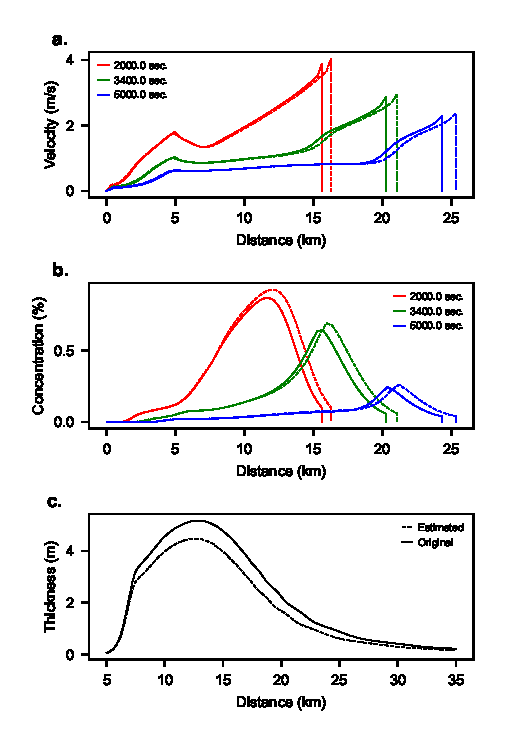
\includegraphics[width=8cm]{fig09.eps}
  \caption{Example of forward model calculation with reconstructed and true parameters. The solid line indicates the calculation result using the predicted parameters, and the dashed line exhibits the results using the true parameters. \textsf{a}. Velocity distribution at 2000, 3500 and 5000 seconds after the flow initiation. \textsf{b}. Total sediment concentration at 2000, 3500 and 5000 seconds after the flow initiation. \textsf{c}. Spatial distribution of bed thickness at 25,000 seconds after the flow initiation. }
  \label{fig:test_example_time_evolution}
\end{figure}


\subsection{Tests for robustness against noise and subsampling on input data}
The test data with various amounts of normal random values are analyzed to verify the robustness of the inverse model. Consequently, even when the standard deviation of the normal random numbers given as measurement errors was set to approximately 200\% of the value of the original data, only a small effect is observed in the normalized RMS of the results of the inverse analysis (Figure \ref{fig:test_noise}). The RMS values gradually increase when the standard deviation of errors exceeds 50\%, but there is no rapid increase in the RMSE of the results at any particular threshold.

\begin{figure}[t]
  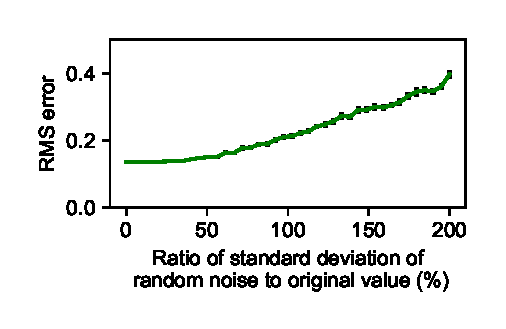
\includegraphics[width=8cm]{fig10.eps}
  \caption{Result of inverse analysis of the test data sets with artificial noise. The values of RMSE are averaged over 20 times iterations. Error bars indicate standard errors of RMSE values.}
 \label{fig:test_noise}
\end{figure}


Similarly, using subsampling data obtained by extracting some of the spatial grids from the original data, we conducted an inverse analysis of the test datasets. The results show that there is little influence on the RMSE values of the inverse analysis of the test datasets when the sampling rate of grids is greater than 1 \% (Figure \ref{fig:test_subsampling}). The RMSE values gradually increased when the sampling rate falls below 1 \%, and RMSE becomes extremely high when the rate drops below 0.4\%.

\begin{figure}[t]
  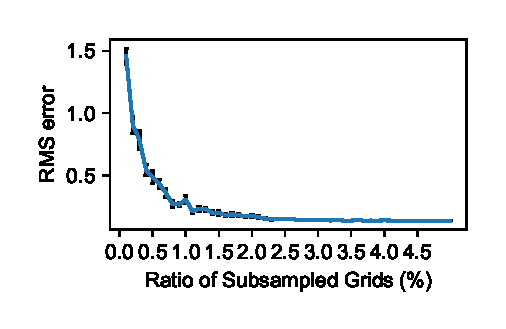
\includegraphics[width=8cm]{fig11.eps}
  \caption{Results of the inverse analysis for the subsampled test data sets. The values of RMSE are averaged over 20 times iterations. Error bars indicate standard errors of RMSE values.}
 \label{fig:test_subsampling}
\end{figure}

